\documentclass{article}

% to compile a preprint version, e.g., for submission to arXiv, add add the
% [preprint] option:
%     \usepackage[preprint]{neurips_2020}

% to compile a camera-ready version, add the [final] option, e.g.:
\usepackage[preprint]{neurips_2020}

% to avoid loading the natbib package, add option nonatbib:
% \usepackage[nonatbib]{neurips_2020}

\usepackage[utf8]{inputenc} % allow utf-8 input
\usepackage[T1]{fontenc}    % use 8-bit T1 fonts
\usepackage{hyperref}       % hyperlinks
\usepackage{url}            % simple URL typesetting
\usepackage{booktabs}       % professional-quality tables
\usepackage{amsfonts}       % blackboard math symbols
\usepackage{nicefrac}       % compact symbols for 1/2, etc.
\usepackage{microtype}      % microtypography
\usepackage[]{algorithm2e}
\usepackage{tikz} 
\usepackage{graphicx}
\usepackage{amsmath}
\usepackage{euler}
\usepackage{wrapfig}

\newcommand{\eat}[1]{#1}

\usetikzlibrary{bayesnet, shapes, arrows, calc, arrows.meta, fit, positioning}
\tikzset{  
    -Latex,auto,node distance =0.3 cm and 1.3 cm, thick,% node distance is the distance between one node to other, where 1.5cm is the length of the edge between the nodes  
    state/.style ={circle, draw, minimum width = 0.9 cm}, % the minimum width is the width of the ellipse, which is the size of the shape of vertex in the node graph  
    point/.style = {circle, draw, inner sep=0.18cm, fill, node contents={}},  
    el/.style = {inner sep=2.5pt, align=right, sloped}  
}  

%%
%% \BibTeX command to typeset BibTeX logo in the docs
% \AtBeginDocument{%
%   \providecommand\BibTeX{{%
%     \normalfont B\kern-0.5em{\scshape i\kern-0.25em b}\kern-0.8em\TeX}}}


%% These commands are for a PROCEEDINGS abstract or paper.
%% \acmConference[CIKM 2020]{29th ACM International Conference on Information and Knowledge Management}{October 2020}{Galway, Ireland}

%%
%% end of the preamble, start of the body of the document source.
\begin{document}

\title{Learning Move Selection Policies from Expert Games}

\eat{
\author{Ralf Herbrich \\
Hasso-Plattner Institute \\
Potsdam, Germany \\
\texttt{ralf.herbrich@hpi.de} \\ 
\And
Alexander Herbrich \\
Technical University of Berlin \\
Berlin, Germany \\
\texttt{aherbrich32@gmail.com}
}
}

\maketitle

\begin{abstract}
Board games have long served as the benchmark for artificial intelligence algorithms. Since the discovery of novel search and machine learning algorithms for Chess (DeepBlue) and Go (AlphaGo), algorithms are capable of playing far beyond the level of the strongest human players. However, these algorithms rely on the ability to either search the game tree much further than any human player could ever attempt or on value function that has been learned from billions of games of self-play and random rollout. In this paper, we introduce a probabilistic model of move selection in the game of chess, which can learn the move selection policy from expert games in the presence of erroneous moves. Using this move selection strategy, we are able to significantly reduce the branching factors of the game tree search, which allows us to build a chess game engine that plays at the level of the strongest chess engine (Stockfish) while consuming considerably less energy.
\end{abstract}

\section{Introduction}

\label{sec:introduction}



\section{Move Selection Model}

\label{sec:introduction}

Our model is based in \cite{stern2006bayesianpatternranking}.

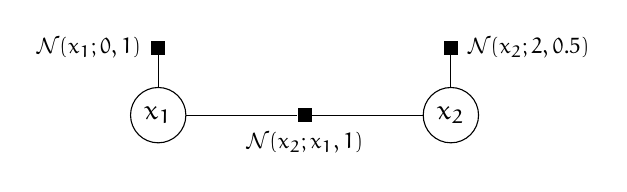
\begin{tikzpicture}
  % Define nodes
  \node[latent] (X_1) {$x_1$};
  \node[latent, right=of X_1, , xshift = 2cm] (X_2) {$x_2$};

  \factor[above = of X_1]{X_1-f}{left:$\mathcal{N}(x_1;0,1)$}{}{};
  \factor[above = of X_2]{X_2-f}{right:$\mathcal{N}(x_2;2,0.5)$}{}{};
  \factor[left = of X_2, xshift=-1cm]{X_1-X_2}{below:$\mathcal{N}(x_2;x_1,1)$}{}{};

  % Define edges
  \factoredge{X_1}{X_1-f}{};
  \factoredge{X_2}{X_2-f}{};
  \factoredge{X_1}{X_1-X_2}{};
  \factoredge{X_2}{X_1-X_2}{};

  % Add plates or other labels if desired
\end{tikzpicture}


\section{Conclusions}

\section*{Acknowledgments}
We would like to thank ...

\appendix

%%
%% The next two lines define the bibliography style to be used, and
%% the bibliography file.
\bibliographystyle{plain}
\bibliography{chess}

\end{document}
% \endinput
